\chapter{Why we can directly subtract a background photon}\label{backgroundSubtract}

\begin{figure}[h!]
    \centering
      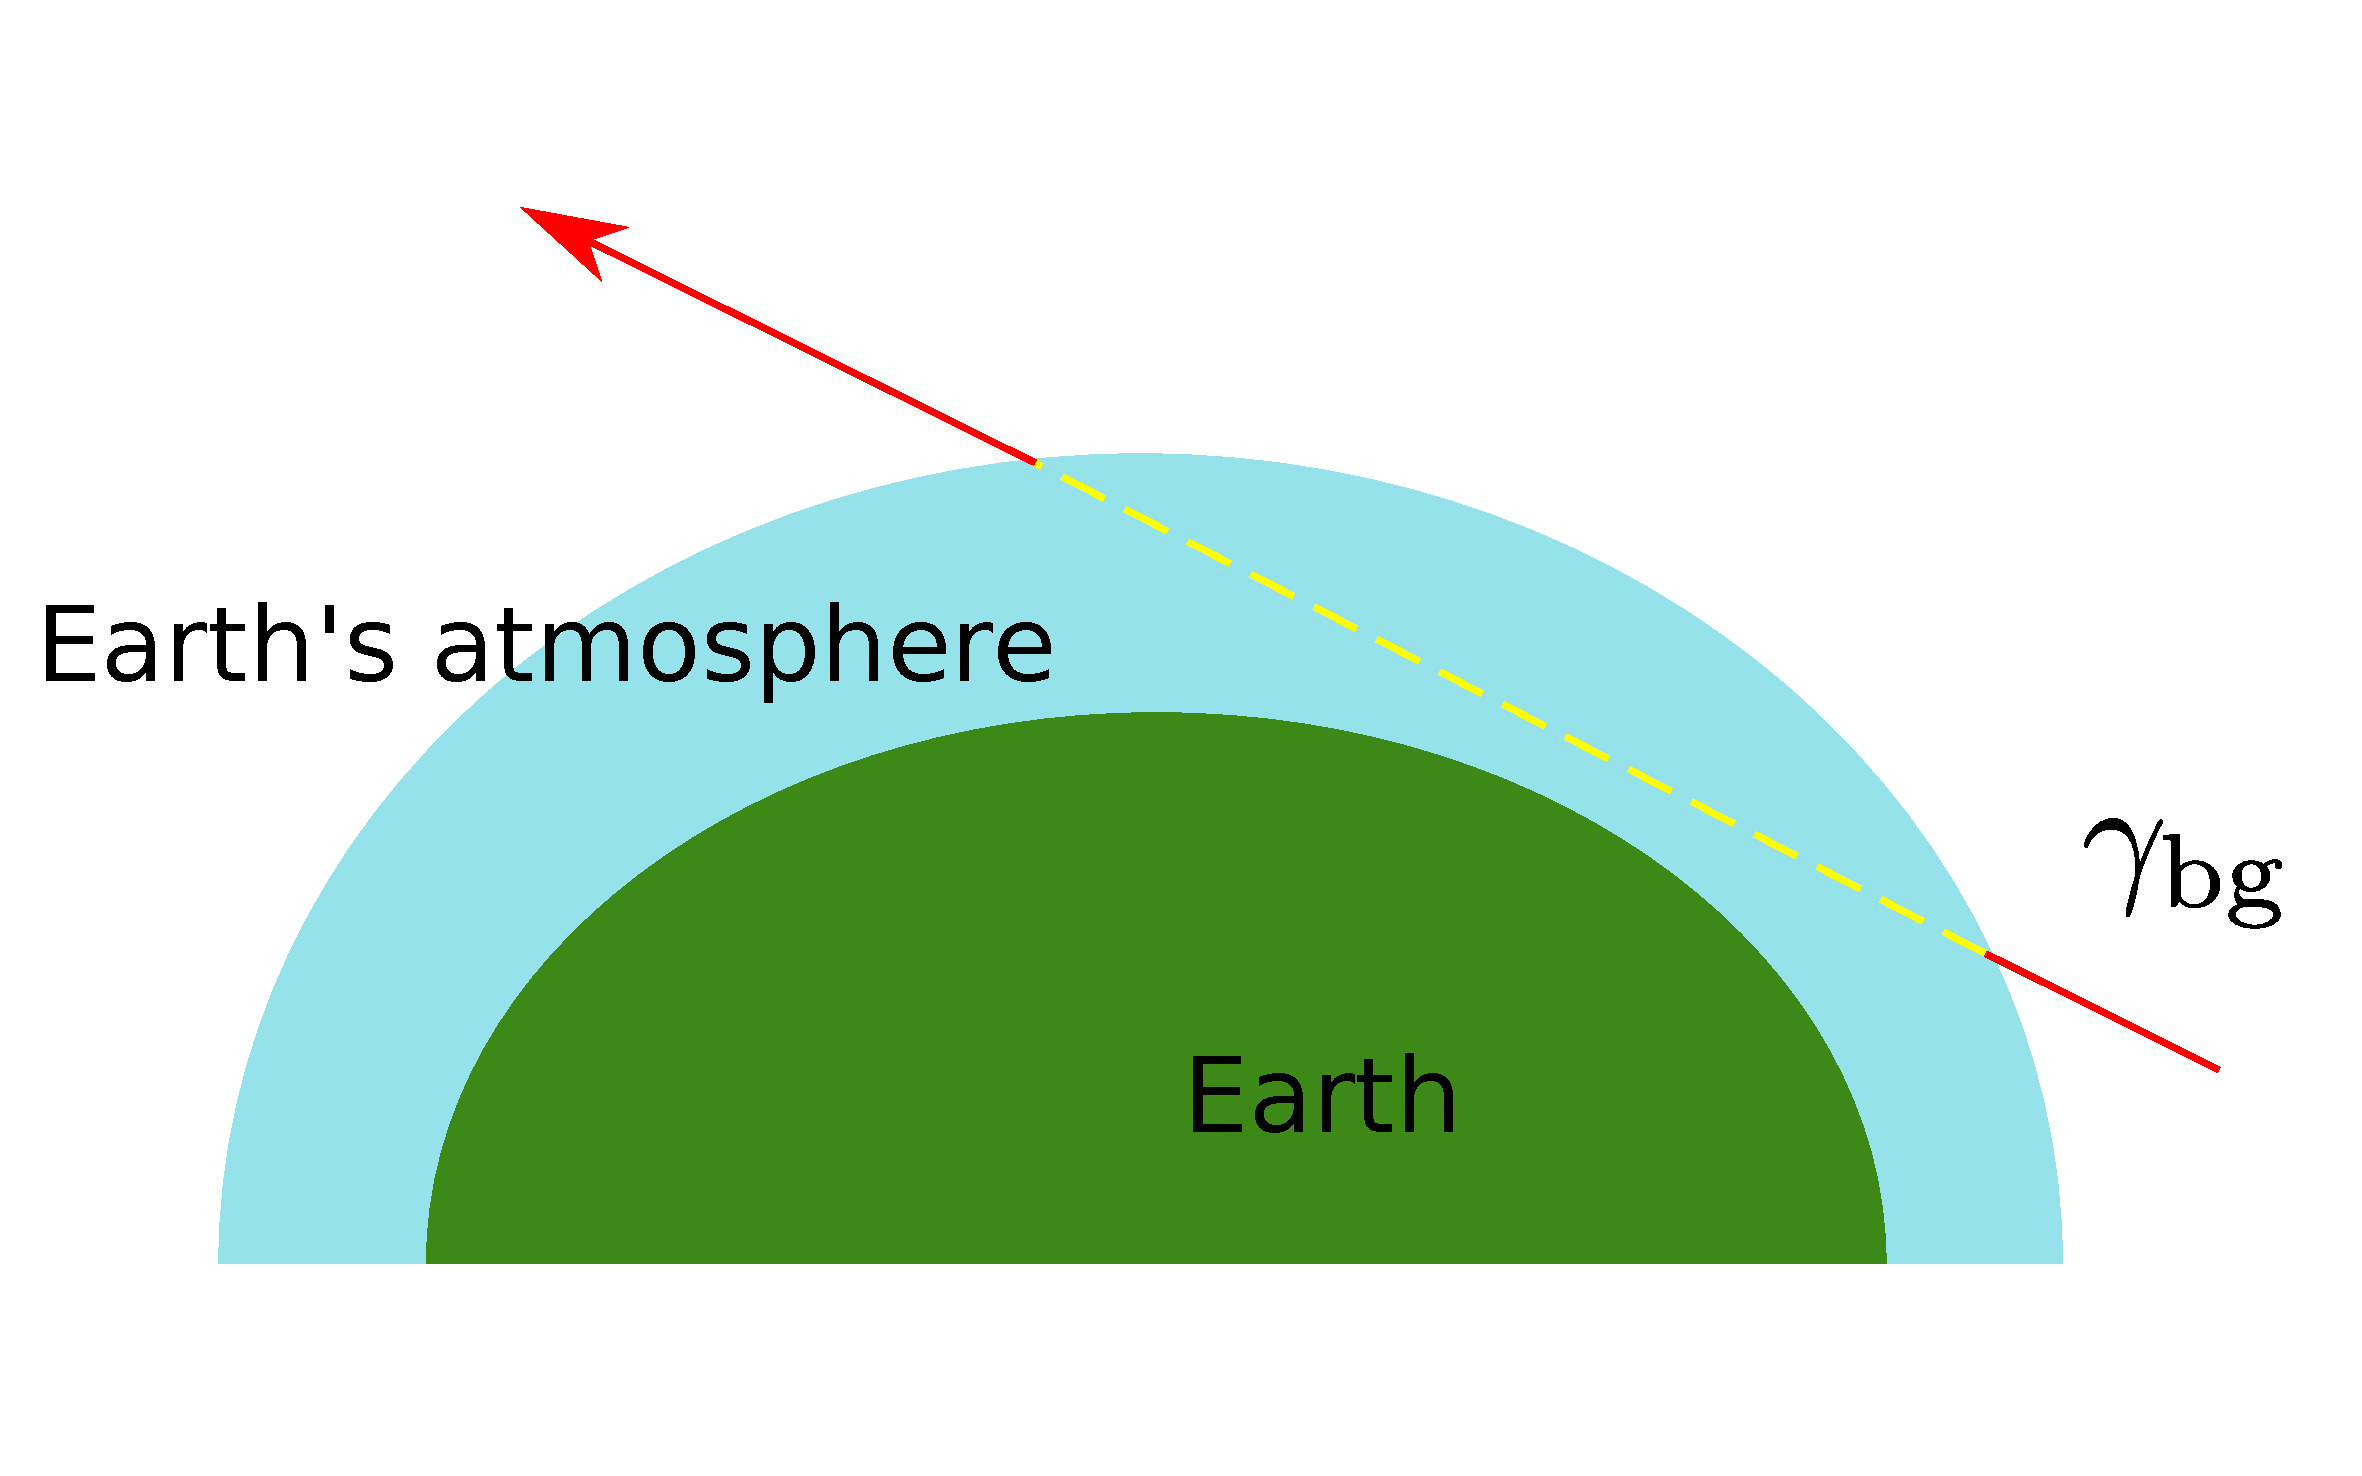
\includegraphics[width=0.7\textwidth]{img/backgroundSubtract}
      \caption{Schematics of $\gamma$-ray propagation from diffusive background}
\end{figure}

Assume Probability of collision with assume ultrarelativistic limit approached to classical concept below
\begin{equation}
    N \equiv N_0 e^{-n\sigma x}
\end{equation}
when
\begin{itemize}
    \item $n$ is a density of air
    \item $\sigma$ is a crossection
    \item $x$ is a propagation length
\end{itemize}
From using crossection data from XCOM:NIST(2010) \cite{XCOMNIST}, we found that collision probability of $\gamma$-ray with nitrogen atom and oxygen atom very similar in energy range of our interest.
If we consider in worse case scenario( longest path and highest density that could happen in atmosphere), we found a passing possibility approach to one more than third order. To sum up, we could straightforwardly remove a background by taking average diffusive background per unit of angle before to apply.


